\PassOptionsToPackage{unicode}{hyperref}
\PassOptionsToPackage{hyphens}{url}
\PassOptionsToPackage{dvipsnames,svgnames,x11names}{xcolor}
\documentclass[
  letterpaper,
  DIV=11,
  numbers=noendperiod]{scrartcl}
\usepackage{xcolor}
\usepackage{amsmath,amssymb}
\setcounter{secnumdepth}{-\maxdimen} % remove section numbering
\usepackage{iftex}
\ifPDFTeX
  \usepackage[T1]{fontenc}
  \usepackage[utf8]{inputenc}
  \usepackage{textcomp} % provide euro and other symbols
\else % if luatex or xetex
  \usepackage{unicode-math} % this also loads fontspec
  \defaultfontfeatures{Scale=MatchLowercase}
  \defaultfontfeatures[\rmfamily]{Ligatures=TeX,Scale=1}
\fi
\usepackage{lmodern}
\ifPDFTeX\else
\fi
\IfFileExists{upquote.sty}{\usepackage{upquote}}{}
\IfFileExists{microtype.sty}{% use microtype if available
  \usepackage[]{microtype}
  \UseMicrotypeSet[protrusion]{basicmath} % disable protrusion for tt fonts
}{}
\makeatletter
\@ifundefined{KOMAClassName}{% if non-KOMA class
  \IfFileExists{parskip.sty}{%
    \usepackage{parskip}
  }{% else
    \setlength{\parindent}{0pt}
    \setlength{\parskip}{6pt plus 2pt minus 1pt}}
}{% if KOMA class
  \KOMAoptions{parskip=half}}
\makeatother
\makeatletter
\ifx\paragraph\undefined\else
  \let\oldparagraph\paragraph
  \renewcommand{\paragraph}{
    \@ifstar
      \xxxParagraphStar
      \xxxParagraphNoStar
  }
  \newcommand{\xxxParagraphStar}[1]{\oldparagraph*{#1}\mbox{}}
  \newcommand{\xxxParagraphNoStar}[1]{\oldparagraph{#1}\mbox{}}
\fi
\ifx\subparagraph\undefined\else
  \let\oldsubparagraph\subparagraph
  \renewcommand{\subparagraph}{
    \@ifstar
      \xxxSubParagraphStar
      \xxxSubParagraphNoStar
  }
  \newcommand{\xxxSubParagraphStar}[1]{\oldsubparagraph*{#1}\mbox{}}
  \newcommand{\xxxSubParagraphNoStar}[1]{\oldsubparagraph{#1}\mbox{}}
\fi
\makeatother

\usepackage{longtable,booktabs,array}
\newcounter{none} % for unnumbered tables
\usepackage{calc} % for calculating minipage widths
\usepackage{etoolbox}
\makeatletter
\patchcmd\longtable{\par}{\if@noskipsec\mbox{}\fi\par}{}{}
\makeatother
\IfFileExists{footnotehyper.sty}{\usepackage{footnotehyper}}{\usepackage{footnote}}
\makesavenoteenv{longtable}
\usepackage{graphicx}
\makeatletter
\newsavebox\pandoc@box
\newcommand*\pandocbounded[1]{% scales image to fit in text height/width
  \sbox\pandoc@box{#1}%
  \Gscale@div\@tempa{\textheight}{\dimexpr\ht\pandoc@box+\dp\pandoc@box\relax}%
  \Gscale@div\@tempb{\linewidth}{\wd\pandoc@box}%
  \ifdim\@tempb\p@<\@tempa\p@\let\@tempa\@tempb\fi% select the smaller of both
  \ifdim\@tempa\p@<\p@\scalebox{\@tempa}{\usebox\pandoc@box}%
  \else\usebox{\pandoc@box}%
  \fi%
}
\def\fps@figure{htbp}
\makeatother

\setlength{\emergencystretch}{3em} % prevent overfull lines

\providecommand{\tightlist}{%
  \setlength{\itemsep}{0pt}\setlength{\parskip}{0pt}}

\KOMAoption{captions}{tableheading}
\makeatletter
\@ifpackageloaded{caption}{}{\usepackage{caption}}
\AtBeginDocument{%
\ifdefined\contentsname
  \renewcommand*\contentsname{Table of contents}
\else
  \newcommand\contentsname{Table of contents}
\fi
\ifdefined\listfigurename
  \renewcommand*\listfigurename{List of Figures}
\else
  \newcommand\listfigurename{List of Figures}
\fi
\ifdefined\listtablename
  \renewcommand*\listtablename{List of Tables}
\else
  \newcommand\listtablename{List of Tables}
\fi
\ifdefined\figurename
  \renewcommand*\figurename{Figure}
\else
  \newcommand\figurename{Figure}
\fi
\ifdefined\tablename
  \renewcommand*\tablename{Table}
\else
  \newcommand\tablename{Table}
\fi
}
\@ifpackageloaded{float}{}{\usepackage{float}}
\floatstyle{ruled}
\@ifundefined{c@chapter}{\newfloat{codelisting}{h}{lop}}{\newfloat{codelisting}{h}{lop}[chapter]}
\floatname{codelisting}{Listing}
\newcommand*\listoflistings{\listof{codelisting}{List of Listings}}
\makeatother
\makeatletter
\makeatother
\makeatletter
\@ifpackageloaded{caption}{}{\usepackage{caption}}
\@ifpackageloaded{subcaption}{}{\usepackage{subcaption}}
\makeatother
\usepackage{bookmark}
\IfFileExists{xurl.sty}{\usepackage{xurl}}{} % add URL line breaks if available
\urlstyle{same}
\hypersetup{
  pdftitle={Problem Set 4: How much do receptors compete?},
  pdfauthor={Jun Allard},
  colorlinks=true,
  linkcolor={blue},
  filecolor={Maroon},
  citecolor={Blue},
  urlcolor={Blue},
  pdfcreator={LaTeX via pandoc}}

\ifXeTeX
\special{pdf:trailerid [ <55dd56121fc11c12abcc50e41411659a> <55dd56121fc11c12abcc50e41411659a> ]}
\fi
\ifPDFTeX
\pdftrailerid{}
\pdftrailer{/ID [ <55dd56121fc11c12abcc50e41411659a> <55dd56121fc11c12abcc50e41411659a> ]}
\fi
\ifLuaTeX
\pdfvariable trailerid {[ <55dd56121fc11c12abcc50e41411659a> <55dd56121fc11c12abcc50e41411659a> ]}
\fi

\title{Problem Set 4: How much do receptors compete?}
\usepackage{etoolbox}
\makeatletter
\providecommand{\subtitle}[1]{% add subtitle to \maketitle
  \apptocmd{\@title}{\par {\large #1 \par}}{}{}
}
\makeatother
\subtitle{Physics 230A/146A --- Biological Physics}
\author{Jun Allard}
\date{}
\begin{document}
\maketitle


A sphere of radius \(R\) that is a perfect absorber, in a far-field concentration \(c_{\infty}\) of particles with diffusion coefficient \(D\), will absorb those particles at a rate \(\lambda_\mathrm{perfect} = 4\pi D R c_{\infty}\).
This implies that a cell of radius \(R\) that were totally covered in receptors for a particular ligand would interact with the ligand at rate \(\lambda_\mathrm{perfect}\).

In reality, only a small fraction of the surface of a cell is covered by receptors for a particular ligand.
In this problem, we compute the interaction rate for a cell with partial absorption.

Assume the cell has radius \(R \sim 10\,\mu\mathrm{m}\) and is covered by \(N\) receptors, each of which is a disk of radius \(a \sim 10\,\mathrm{nm}\).
We make use of an approximation method that assumes there is a radius \(r=R_I\) that is sufficiently far from the cell surface, compared to the size of a receptor, that it appears infinitely far at the scale of this receptor, but is sufficiently close to the cell surface that, from far away, it appears approximately the same size as the cell.
(By analogy, the planet Earth is of radius \(R\), and people on its surface are of size \(a\ll R\).
Let \(R_I\) be the radius of the Earth's stratosphere: At the scale of a person, \(R_I\) is very far from the person, yet at the scale of the solar system, the radius of the Earth with or without the stratosphere are indistinguishable, i.e., \(R_I \approx R\).)

\begin{center}
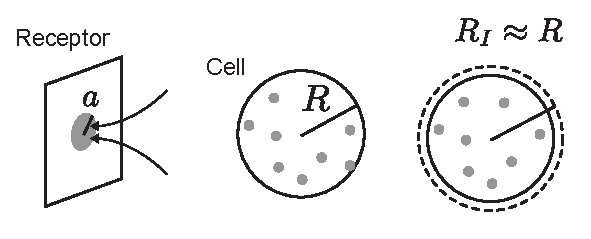
\includegraphics[width=9cm,height=\textheight,keepaspectratio]{fig_receptor-competition.pdf}
\end{center}

\begin{enumerate}
\def\labelenumi{\roman{enumi}.}
\item
  An infinite sheet that is no-flux, except for a perfect absorbing disk of radius \(a\), absorbs particles at rate \(\lambda_\mathrm{disk} = 4D a c_{I}\) where \(c_I\) is the concentration sufficiently far from the disk.
  Therefore the rate at which \(N\) disks absorb particles is \(\lambda_{N} = 4D N a c_{I}\).

  At \(r=R_I\), what is the average flux (in particles per time per unit area) of particles, \(\langle J(R_I)\rangle\)?
  The answer should involve \(c_I\) (which is unspecified at this stage in the calculation).
\item
  At the scale larger than the cell, the concentration \(c(r)\) satisfies the steady-state diffusion equation

  \[
  0 = D \nabla^2 c.
  \]

  This equation has 3 boundary conditions:

  \[
  \begin{aligned}
  c(r) &\rightarrow c_{\infty} \qquad \text{as} \qquad r\rightarrow \infty\\
  c(R_I) &= c_I, \\
  J(R_I) &= - D \nabla c.
  \end{aligned}
  \]

  Note that this type of ODE usually requires 2 boundary conditions, but since \(c_I\) is unspecified, here 3 boundary conditions are needed.
  Solve the system by making two approximations: First, assume \(J(R_I) = \langle J(R_I)\rangle\) from part (i).
  (This corresponds to assuming the stratosphere is far from the receptors.)
  Second, assume \(R=R_I\) (This corresponds to assuming the stratosphere is close to the surface).
\item
  What is the rate \(\lambda\) at which particles arrive at the surface?
  This will depend on \(N\).
  You should find that as \(N\rightarrow\infty\), the rate \(\lambda\rightarrow\lambda_\mathrm{perfect}\), the rate for a perfectly absorbing sphere.
\item
  How many receptors \(N\) are needed to obtain half the perfect-absorption rate?
  At this value of \(N\), what fraction of the cell's surface is covered by receptors?
  You may use \(R \sim 10\,\mu\mathrm{m}\) and \(a \sim 10\,\mathrm{nm}\).
\end{enumerate}

This method of approximation, by assuming an intermediate distance between two scales, is an example of the Applied Mathematics technique called \emph{matched asymptotics}.




\end{document}
